\documentclass{article}

% To use unicode character
\usepackage[utf8]{inputenc}

% For clickable links
\usepackage{hyperref}

% To control margins
\usepackage[margin=1.5in]{geometry}

% For bibliography
\usepackage[square,numbers]{natbib}
\bibliographystyle{abbrvnat}

% For pictures
\usepackage{graphicx}

% To typeset math
\usepackage{amsthm}
\usepackage{amsmath}
\usepackage{amsfonts}
\usepackage{bbm} % For indicator function

% Figure
\usepackage{caption}
\usepackage{subcaption}

% To typeset code
\usepackage{listings}

% Well, it's in the name
\usepackage{algorithm}
\usepackage[noend]{algpseudocode}


\DeclareMathOperator*{\argmax}{arg\,max}

% ====================================
\title{On Upper-Confidence Bound Policies for Non-Stationary Bandit Problems}
\author{Maxence Giraud, Mathis Demay}
\date{2020}

\begin{document}

\maketitle

\begin{abstract}

	In this report we sum up the work of Garivier et al. \cite{garivier2008upperconfidence} and try to extend their work to new possibilities. This paper is about finding an algorithm for the non-stationary bandit problem. The authors study two algorithms, both based on \textit{Upper-Confidence Bound}(UCB) policies. The first, already existing algorithm is \textit{Discounted-UCB}(D-UCB), and they propose another one, \textit{Sliding-Window UCB}(SW-UCB). We implemented both policies and try to compare to two new variants we came up with of \textit{Sliding-Window UCB}(SW-UCB).
	
\end{abstract}

\section{Introduction}

	\subsection{Multi armed bandits and UCB1 algorithm}

		The problem of stationary Multi-Armed Bandit (MAB) models a learning situation where the learner, called the \textit{bandit} goes through successive steps, and at each step, can choose between the advice of different advisors, called the \textit{arms}. Then it receives a reward, depending on how far the arm it chose was of good advice. This problem is said to be \textit{stationary} because the rewards of the arms follow a distribution constant over time.

The crux of this situation is to trade-off between exploiting the arms known to be good, and exploring the others, in case they would be of good advice too.\\

[TODO] Define how many notions ? Regret and so on []

Formally, we consider a bandit with $K$ arms, referred to as $[\![1,K]\!]$. At each time $t$, the learner has to choose an arm $I_t \in [\![1,K]\!]$. This is done following a given policy $\pi$, which can be deterministic or random. Then, it receives a reward $X_t(I_t)$. In the stationary case, we suppose that for each $i \in [\![1,K]\!]$, the sequence $\{X_t(i)\}_{t \geq 1}$ of rewards of arm $i$ is made up of independent and identically distributed (i.i.d.) variables. This means the distribution of rewards of arm $i$ is constant over time. Thus we can define $\mu(i)$ to be the expected reward at each time step, without a dependence on $t$.

The general aim is to find a policy which gets the largest expected reward. The optimal one is denoted by $\pi^*$, with reward $\mu^*=\underset{1\leq i \leq K}{\max} \mu(i)$. It is obtained by constantly playing arm $i^* = \underset{1\leq i \leq K}{\argmax}\ \mu(i)$.

In order to assess the performance of a policy we define the regret of a policy, which measures how far it strays from the optimal one: $R(T,\pi)=\mathcal{E}\left[\sum_{t=1}^T \mu^* - \mu(I_t) \right]$.

Finally, we define $N_t(i)=\sum_{s=1}^t \mathbbm{1}(I_s=i)$ to be the number of times arm $i$ has been played until time $t$.\\

A well-known, efficient class of policies is that of the UCB	algorithms, which consist in playing, at each step $t$, deterministically, the arm $i$ which maximizes the upper bound $B(t,i)$ of a confidence interval for its expected reward $\mu(i)$.
Among these, a particularly famous one is known as \textit{UCB-1}, and is described in Algorithm \ref{alg:ucb1}.

\begin{algorithm}
    \caption{UCB1}
	\label{alg:ucb1}
    For t from 1 to $K$, play arm $I_t = t$ \\
    For t from $K$+1 to $T$, play arm 
    $$ I_t = \argmax_{1\leq i \leq K} \bar X_t(i) + c_t(i)$$
\end{algorithm}


In UCB-1, one sets $B(t,i)=\bar{X}_t(i)+c_t(i)$, where $\bar{X}_t(i)=\frac{1}{N_t(i)}\sum_{s=1}^t X_s(i)\mathbbm{1}(I_s=i)$ takes the past into account, constituting an exploitation term, and $c_t(i)$ is a \textit{padding function}, meant to be an exploration term. Note that the two algorithms studied in the following can be formulated the same way, the only change dwelling in this padding function. Here the authors propose $c_t(i)=B\sqrt{\xi \log(t)/N_t(i)}$, with $B$ an upper bound of the rewards, and $\xi>0$ a hyperparameter.



	\subsection{Non Stationary Bandits}

		The work discussed in this paper is focused on Non-Stationary bandit, as of now we have only seen Stationary bandit. In this problem the must decide which arm to play with the same reward system as in the classic Multi-armed bandit problem but facing the possibility of a changing environment.\\

This problem can be expressed in the following way. The rewards $X_s(i)$ of an arm $i$ is modeled by an independant sequence of random variables from a distribution that may change across time.\\

Garivier et al. focused their work on abruptly changing environment, meaning that the distributions of rewards remain constant during periods and change at unknown time instants called \textbf{breakpoints}. Other non Stationary bandits problem exist where the distributions of the rewards are changed continuously but are not the topic of this paper.\\

It is straighforward that standard policies such as UCB reviewed in the last subsection are not appropriate for this kind of environment, this is why the authors introduce two new algorithms : Discounted UCB and Sliding Window UCB which we are going to discuss in the rest of this report.

\section{Discounted UCB}
	The first algorithm studied here was initially proposed by Kocsis and Szepesvári in 2006 \cite{Kocsis06banditbased} and is called Discounted UCB. In order to estimate the instantaneous expected reward, the policy averages the past reward with a discoud $\gamma$ which decrease exponentionally with time (the older a reward is, the less significant it is).  The policy algorithm is described in \ref{alg:d_ucb}. We can notice without much effort that if the discout factor $\gamma$ is set to 1, the discounted UCB boils down the original UCB algorithm.\\

\begin{algorithm}[ht]
    \caption{Discounted UCB}
    \label{alg:d_ucb}
    For t from 1 to $K$, play arm $I_t = t$ \\
    For t from $K$+1 to $T$, play arm 
    $$ I_t = \argmax_{1\leq i \leq K} \bar X_t(\gamma,i) + c_t(\gamma,i)$$
\end{algorithm}

Where
\begin{align}
\bar{X}(\tau, i) &= \frac{1}{N_t(\tau, i)}
\sum_{s=t-\tau+1}^t \gamma^{t-s}X_s(i)\mathbbm{1}(I_s=i)\\
N_t(\gamma, i) &= \sum_{s=t-\tau+1}^t \gamma^{t-s}\mathbbm{1}(I_s=i)\\
c_t(\tau, i) &= 2B\sqrt{\frac{\xi \log(n_t(\gamma))}{N_t(\gamma,i)}}\\
n_t(\gamma) &= \sum_{i=1}^K N_t(\gamma,i)
\end{align}

We call in this context $c$ the dicounted padding function and $\bar X$ represent the discounted empirical average.\\
As this algorithm seems to be more fitted in continuous changing environment (because of the $\gamma$), they authors propose another method that would be though to work in more abruptly changing environments.\\

The authors propose an in depth analysis of the discounted UCB policy,  The complete list of Theorems and proofs can be found in the original paper by Garivier and Moulines \cite{garivier2008upperconfidence}. We won't focus our report on those findings which mostly consist of complex bounds on some values of the policy which are not easy to understand the underlying significance.

\section{Sliding Window UCB}

	After reviewing the Discounted UCB algorithm, the authors propose a new algorithm called Sliding Window UCB. This time instead of relying on some discounted values of past reward, the policy is only insterested in the last $\tau$ rewards. Conceptually this algorithm is very much suited to the non-stationary scenario as it will disregard old drawings of arms. The full algorithm is described in Algorithm \ref{alg:sw_ucb}.\\

\begin{algorithm}
    \caption{Sliding Window UCB}
    \label{alg:sw_ucb}
    For t from 1 to $K$, play arm $I_t = t$ \\
    For t from $K$+1 to $T$, play arm 
    $$ I_t = \argmax_{1\leq i \leq K} \bar X_t(\tau,i) + c_t(\tau,i)$$
\end{algorithm}

Again, $\beta(t,i)=\bar{X}_t(i)+c_t(i)$.
However, about the definition of $\bar{X}$ given in the paper, we reckon there is a problem in the definitions. In the definition of $X$ there is an $N_t(\gamma, i)$ but no $\gamma$ in the sum, however $\gamma$ appears in the sum of $N_t$. Then the definition of $\bar{X_t}$ is not homogeneous in terms of $\gamma$. Also, in the definition of $c_t$, $N_t$ appears with a parameter $\tau$, not $\gamma$. Also, the sum in $N_t$ begins at $t=1$, not considering the same amount of terms as $X_t$. We concluded the definitions of $\bar{X_t}$ and $c_t$ are right but $N_t$ is a wrong copy-paste. Then we propose the following definitions:
\begin{align}
\bar{X}(\tau, i) &= \frac{1}{N_t(\tau, i)}\sum_{s=t-\tau+1}^t X_s(i)\mathbbm{1}(I_s=i) \\
N_t(\gamma, i) &= \sum_{s=t-\tau+1}^t \mathbbm{1}(I_s=i) \\
c_t(\tau, i) &= B\sqrt{\frac{\xi \log(min(t, \tau))}{N_t(\tau,i)}}
\end{align}

These definitions drop $\gamma$, taking into account the fact that they say their variant is 'more abrupt [than \textit{D-UCB}]'. However, it could be interesting to see if the combination of the discount factor and the sliding window is interesting, but they unfortunately don't tackle this question.

We eventually found in \cite{slidesGarivier} that our definition of $N_t$ was good.

Also, they don't deal with the case of an arm which has not been selected in the $\tau$ last steps. In the current formulation, this leads to $N_t(\gamma, i)=0$ and to a division by $0$ in the definition of $\bar{X}(\tau, i)$.

[TODO] More properties ?[]

\section{Experiments} \label{sec_expes}
	
	\subsection{Variants of Sliding Window UCB}
	
		In order to deal with the ill-defined SW-UCB, we try $3$ possibilities for this algorithm. Anyway, whether the definition is wrong or not is not a big deal anymore; we find it interesting to explore these $3$ possibilities.

First we choose to work with $\tau > K$. This hypothesis may sound a little arbitrary, however it is coherent in the sense that looking at less time steps than the actual number of arms does not look like a very reliable solution. The exploitation part has to look at several past events in order to be relevant. In that sense we can also say that $\tau$ should be a multiple of $K$, say $5K$ for example. 

Then, with this hypothesis $\tau > K$ we can do something

The first possibility is to 

	\subsection{Our experiments}

		The code for all the experiments described in this section are available at the following link : \url{https://github.com/MaxenceGiraud/ucb-nonstationary}.

We performed three different experiments using the five algorithms described in this paper. The first one is the original UCB-1 used as a baseline for all the experiments. The second one is Disounted UCB, and the last three are the Sliding Window UCB described by Garivier et al. \cite{garivier2008upperconfidence} and the two variants we talked about in the last section.\\
The parameters of the policies were tuned as Garivier et al. did. This means with for all algorithms $\xi = 0.5$, $\gamma = 1 - \frac{1}{4\sqrt{T}}$ and $\tau = 4 \sqrt{K \log(T)}$. As an example for $T=1000$ and $K=3$, $\tau = 18$ and $\gamma = 0.992$.\\

The first experiment consists of a simple stationary problem with three Gaussian with means respectively 0.2, 0.3 and 0.4. The results are displayed on figure \ref{fig:statio}. As we expected the original UCB performed much better than all the other algorithms. One justification of the poor performance in the case of the main policy of interest Sliding Window UCB, can be that it has to draw each arm at least $T/\tau$ times and so even if one arm is consistently better than the others, it will draw it consequent number of times.\\

\begin{figure}[ht]
    \centering
    \begin{subfigure}{.6\textwidth}
      \centering
      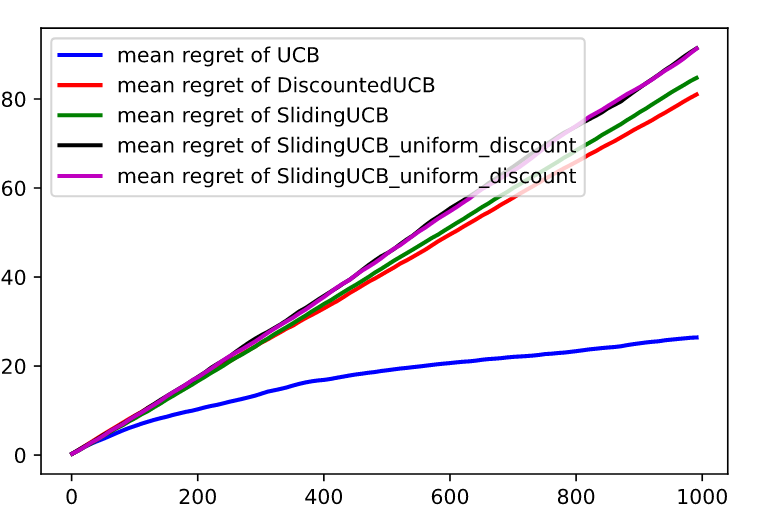
\includegraphics[width=.8\linewidth]{img/statio.png}
      \caption{Stationary Bandit}
      \label{fig:statio}
    \end{subfigure}%
    \begin{subfigure}{.6\textwidth}
      \centering
      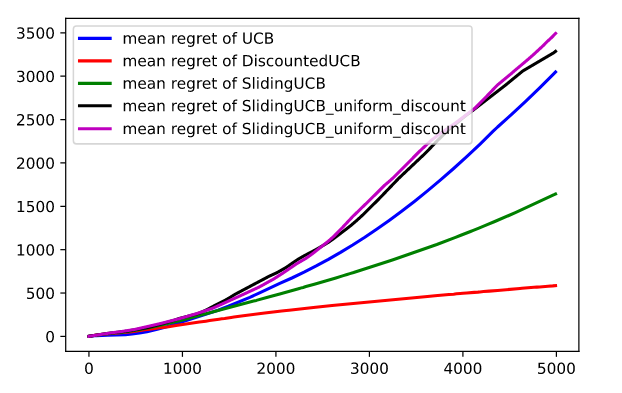
\includegraphics[width=.8\linewidth]{img/continuous.png}
      \caption{Continuously changing MAB}
      \label{fig:conti}
    \end{subfigure}
    \begin{subfigure}{.6\textwidth}
        \centering
        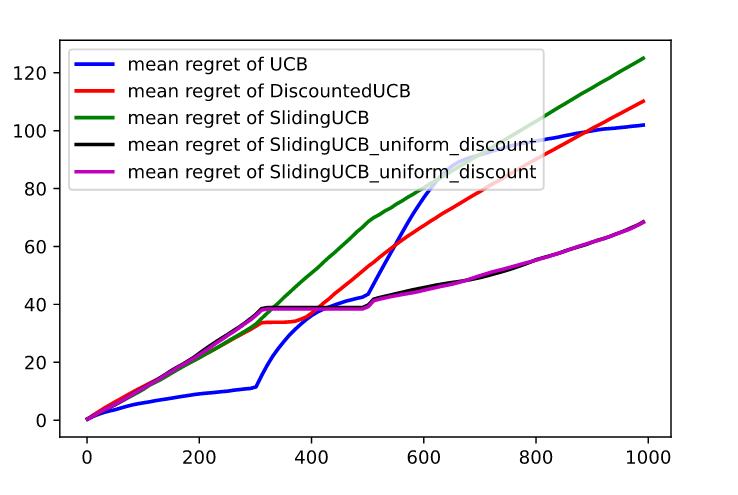
\includegraphics[width=.8\linewidth]{img/abrupt.png}
        \caption{Abrubtly changing MAB}
        \label{fig:abrupt}
      \end{subfigure}
\end{figure}


The second experiment consists of a continuously changing environment. We kept two arms stationary which are Gaussians of means 0.2 and 0.7 while the third is a Gaussian with a mean dependant of the time t: $0.4 + \frac{t}{T}$. The results are reported in figure \ref{fig:conti}.\\
Again as expected, the best performing policy is the Discounted UCB which is design for this kind of environment. We also found as in the studied paper that the Sliding UCB is still performing quite well on this problem, while our two variants fail and do worse than a standard UCB.\\

The last experiment is the main study of the paper, is the abruptly changing environment. It is modeled as follows: two arms do not change over time and are represented by Bernouilli with parameters respectively 0.5 and 0.4. And a third arm that for $T < 300 $ and $T > 500$ it is modeled as a Bernouilli with probability equals to 0.1 while in the interval it is 0.9. The results of this third experiment are reported in figure \ref{fig:abrupt}.\\
Here the best performing algorithm is actually our first variant (the Sliding UCB with Uniform Discount) while Sliding UCB is the worse performing one. We cannot firmly conclude over these results as firstly they contradict the ones from the paper, and secondly due to a lack of machines that could perform long tasks ($T>10000$) a sufficient number of times for the experiment to be statistically conclusive.

\section{Critique}
	
	We have several remarks regarding the paper.

The obvious lack of rereading of the definition of \textit{SW-UCD} is definitely a pity, because it is at the root of their main contribution and the subsequent analysis and other paragraphs which follow.

In general, the paper is not very clear. We soon get lost into computational details, without the authors helping us get the big picture out of it. At least, this is what we think, comparing with other papers. For example, if they had described the idea behind SW-UCB more, we might have understood their point.  This difficulty to follow is enhanced by the length of their demonstrations. However they tried to make them easier to follow by breaking them down into different steps.

Still, the analyses of the algorithms are exhaustive.

They could have compared the performances of UCB1 and the others on the stationary environment.

Concerning the experiments, for D-UCB and SW-UCB they took the hyperparameters tuned to the very problem they are working on, and for UCB1 they took theoretical values from another paper. This is criticizable. 

Still, for reproducibility they gave parameters so it is reproducible, more than in many other papers. We couldn't reproduce their results, but this is more likely due to other reasons (such as errors in the code, maybe).

\section{Conclusion}

	The main contribution of the paper is the Sliding Window-UCB algorithm, along with the analysis of the latter and Discounted-UCB.\\

Our main critique is that the paper is not always clear.\\
According to them, D-UCB and SW-UCB perform well on changing environments, unlike UCB1. In practice, we confirmed that UCB1 is the best on constant environments, but in abruptly changing environments it is harder to tell.

\bibliography{nsucb}

\end{document}
